\documentclass[pra,12pt]{revtex4}
\usepackage{amsmath}
\usepackage{amssymb}
\usepackage{graphicx}
\usepackage{color}
\usepackage[pdfborder={0 0 0},colorlinks=true,linkcolor=blue]{hyperref}

\def\ket#1{\left|#1\right\rangle}
\def\bra#1{\left\langle#1\right|}
\def\braket#1{\left\langle#1\right\rangle}

\setlength{\parindent}{0pt}

\renewcommand{\baselinestretch}{1.0}
\setlength{\parskip}{0.07in}

\begin{document}

\begin{center}
{\large \textbf{Appendix A: Partial Wave Analysis}}
\end{center}

In this Appendix, we describe the method of \textbf{partial wave
  analysis}, which can be used to solve a specific class of 3D
scattering problems: those with a \textit{spherically symmetric}
scattering potential, $V(r)$, which depends only on the radial
distance $r = \sqrt{x^2 + y^2 + z^2}$ and not on direction.  This
typically describes a situation where a point particle or
spherically-symmetric object sits at the coordinate origin,
$\mathbf{r} = 0$, and is bombarded by incident particles.

\section{Spherical waves}
\label{sec:spherical}

We begin by considering ``exterior'' solutions to the Schr\"odinger
wave equation.  Far from the scatterer, where $V(r) \rightarrow 0$,
the Schr\"odinger wave equation can be rearranged into
$$\Big(\nabla^2 + k^2\Big) \psi(\mathbf{r}) = 0,\;\;\;\mathrm{where}\;\;k = \sqrt{2mE/\hbar^2},$$
which is called the \textbf{Helmholtz equation}.  We emphasize that
$E$ is to be treated as a tunable parameter in the differential
equation, not as an eigenvalue in an eigenproblem.  For the moment, we
will not specify the boundary conditions, and look instead for a
general set of solutions for a given $E$ (and hence $k$).

In spherical coordinates $(r,\theta,\phi)$, the Helmholtz equation has
the explicit form
$$\frac{1}{r^2}\frac{\partial}{\partial r}\left(r^2\frac{\partial \psi}{\partial r}\right) + \frac{1}{r^2\sin\theta}\frac{\partial}{\partial\theta}\left(\sin\theta\frac{\partial\psi}{\partial\theta}\right)+\frac{1}{r^2\sin^2\theta}\frac{\partial^2\psi}{\partial\phi^2} + k^2\psi(r,\theta,\phi) = 0.$$
There is a standard procedure for solving this partial differential
equation.  The first step is to perform a separation of variables, and
look for solutions of the form
$$\psi(r,\theta,\phi) = A(r) Y_{\ell m}(\theta,\phi),$$
where $A(r)$ is a function to be determined and $Y_{\ell
  m}(\theta,\phi)$ is a special function known as a
\href{https://en.wikipedia.org/wiki/Spherical_harmonics}{spherical
  harmonic}.  Spherical harmonics are functions designed specifically
to represent the angular dependence of solutions with definite angular
momenta.  In the context of quantum mechanics, $\ell$ and $m$ are the
quantum numbers representing the total angular momentum and the
$z$-component of the angular momentum.  It can be shown that the
indices $\ell$ and $m$ must be integers satisfying $\ell \ge 0$ and
$-\ell\le m \le \ell$, in order for $Y_{\ell m}(\theta,\phi)$ to be
periodic in $\phi$ and regular at the poles of the spherical
coordinate system.  Once this form for $\psi(r,\theta,\phi)$ is
substituted into the Helmholtz equation, it can be shown that the
radial factor $A(r)$ must satisfy the following ordinary differential
equation (a variant of the Bessel equation):
$$\frac{d}{dr}\left(r^2\frac{dA}{dr}\right) + \Big[k^2r^2 - \ell(\ell+1)\Big] A(r) = 0, \;\;\;\ell \in \mathbb{Z}_0^+,$$
Note that $m$ does not appear in this equation, so $A(r)$ depends on
$\ell$, but \textit{not} on $m$.

The above equation has two linearly independent real solutions,
$j_\ell(kr)$ and $y_\ell(kr)$, which are called \textbf{spherical
  Bessel functions}.  Most scientific computing packages provide
functions to calculate these; Scientific Python, for example, has
\href{https://docs.scipy.org/doc/scipy/reference/generated/scipy.special.spherical_jn.html}{\texttt{scipy.special.spherical\_jn}}
and
\href{https://docs.scipy.org/doc/scipy/reference/generated/scipy.special.spherical_yn.html}{\texttt{scipy.special.spherical\_yn}}.
Various spherical Bessel functions are plotted below:

\vskip 0.5cm
\begin{center}
  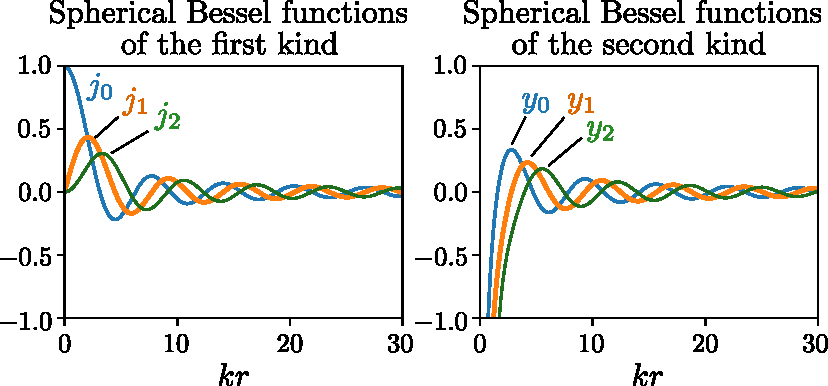
\includegraphics[width=0.63\textwidth]{spherical_bessel}
\end{center}

Note that the spherical Bessel functions of the second kind,
$y_\ell(kr)$, diverge at $kr\rightarrow 0$.  This does not bother us,
since we're interested in solutions defined in the exterior region,
away from the coordinate origin.

For large values of the input, the spherical Bessel functions have the
limiting forms
$$\begin{aligned}j_\ell(kr)\; &\overset{kr\rightarrow\infty}{\longrightarrow} \; \frac{\sin(kr-\frac{\ell\pi}{2})}{kr} \\ y_\ell(kr)\; &\overset{kr\rightarrow\infty}{\longrightarrow} \; - \frac{\cos(kr-\frac{\ell\pi}{2})}{kr}.\end{aligned}$$
Since we are interested in incoming and outgoing spherical waves, it
is convenient to define
$$h_\ell^\pm(kr) = j_\ell(kr) \pm i y_\ell(kr).$$
This is called a \textbf{spherical Hankel function} of the first kind
($+$) or second kind ($-$).  It is a complex function that solves the
same differential equation, but has the limiting form
$$h_\ell^\pm(kr)\; \overset{kr\rightarrow\infty}{\longrightarrow} \; \pm \frac{\exp\left[\pm i(kr-\frac{\ell\pi}{2})\right]}{ikr}.$$
We can use this to write down a solution to the Helmholtz equation, in
the form
$$\Psi_{\ell m}^\pm(\mathbf{r}) = h_{\ell}^\pm(kr) \,Y_{\ell m}(\theta,\phi),$$
which describes a spherical wave that is outgoing ($+$) or incoming
($-$), with a definite angular momentum described by quantum numbers
$\ell$ and $m$.

Because the Helmholtz equation is linear, any linear combination of
spherical waves, with various values of $(\ell,m)$, is also a solution:
$$\psi(\mathbf{r}) = \sum_\pm \sum_{\ell = 0}^\infty \sum_{m = - \ell}^\ell c_{\ell m}^\pm \Psi_{\ell m}^\pm(\mathbf{r}).$$
Moreover, it can be shown that the spherical waves form a complete
solution basis.  In other words, any solution to the 3D Helmholtz
equation within the exterior region can be written in the above form,
for some choice of complex coefficients $c_{\ell m}^\pm$.  Note, by
the way, that the spherical waves are appropriately normalized so that
the flux associated with each term is directly proportional to
$|c_{\ell m}^\pm|$.

\section{The scattering matrix}

For a given scattering problem, the exterior wavefunction is described
by the complex numbers $\{c_{\ell m}^+\}$ and $\{c_{\ell m}^-\}$.
These two sets of coefficients cannot, however, be independent of each
other.  For some fixed $V(\mathbf{r})$ and $E$, suppose there is an
incoming spherical wave with a specific angular momentum, say $c_{\ell
  m}^- = 1$ for some choice of $(\ell,m)$.  After being scattered, the
quantum particles must flow back out to infinity; the scattered
wavefunction can be described by a set of outgoing spherical wave
coefficients, $\{c_{\ell' m'}^+\;|\, \ell' \ge 0, \ell' \le m' \le
\ell'\}$.  We can repeat this for different values of incoming
$(\ell,m)$, each time getting another set of outgoing coefficients.

Since the Schr\"odinger wave equation is linear, the principle of
superposition states that linear combinations of scattering solutions
are also valid solutions---i.e., solutions to the same Schr\"odinger
wave equation, with the same $V(\mathbf{r})$ and $E$.  This implies
that if we supply an \textit{arbitrary} set of incoming coefficients
$\{c_{\ell m}^-\}$, the outgoing coefficients must be determined by a
linear relation of the form
$$c_{\ell m}^+ = \sum_{\ell'm'} S_{\ell m, \ell' m'} \;c_{\ell' m'}^-.$$
To make the notation a bit clearer, let us write this as
$$c_{\mu}^+ = \sum_{\nu} S_{\mu \nu} \, c_{\nu}^-.$$
Here, each $\mu$ or $\nu$ denotes a pair of angular momentum quantum
numbers $(\ell,m)$, and is called a \textbf{scattering channel}.  The
matrix $S$ is called a \textbf{scattering matrix}, and its components
$S_{\mu\nu}$ can be calculated from $V(\mathbf{r})$ and $E$.  Knowing
$S$, we can calculate the scattered wavefunction produced by any set
of incident waves.

In the discussion so far, we have not specified how the ``incoming''
and ``outgoing'' waves are related to the ``incident'' and
``scattered'' waves of a scattering experiment.  Let us now consider
an incident plane wave, $\psi_i(\mathbf{r}) = \Psi_i
\exp(i\mathbf{k}_i\cdot \mathbf{r})$, where $|\mathbf{k}_i| = k$.
This introduces an important complication: relative to the coordinate
origin, a plane wave is neither purely ``incoming'' nor ``outgoing''!
There is a mathematical identity stating that
$$\begin{aligned}e^{i\mathbf{k}_i \cdot \mathbf{r}} &= \sum_{\ell=0}^\infty \sum_{m=-\ell}^\ell 4 \pi j_{\ell}(kr) e^{i\ell\pi/2} \, Y_{\ell m}^*(\hat{\mathbf{k}}_i) \, Y_{\ell m}(\hat{\mathbf{r}})\\ &= \sum_{\ell=0}^\infty \sum_{m=-\ell}^\ell 2 \pi \left[h_{\ell}^+(kr) + h_{\ell}^-(kr)\right] e^{i\ell\pi/2} \, Y_{\ell m}^*(\hat{\mathbf{k}}_i) \, Y_{\ell m}(\hat{\mathbf{r}}).\end{aligned}$$
Here, $\hat{\mathbf{k}}_i$ denotes the angular components (in
spherical coordinates) of the incident wave-vector $\mathbf{k}_i$,
while $\hat{\mathbf{r}}$ likewise denotes the angular components of
the position vector $\mathbf{r}$.  Therefore, the plane wave can be
decomposed into a superposition of incoming and outgoing spherical
waves, with the wave coefficients
$$c^{\pm}_{i, \ell m} = 2 \pi e^{i\ell\pi/2} \, Y_{\ell m}^*(\hat{\mathbf{k}}_i)\; \Psi_i.$$
As described in Chapter 1, the total wavefunction in a scattering
problem is the sum of the incident wavefunction $\psi_i(\mathbf{r})$
and the scattered wavefunction $\psi_s(\mathbf{r})$.  The latter must
be a superposition of outgoing spherical waves; let us denote the
coefficients by $c^+_{s,\ell m}$.  The scattering matrix relation can
be then re-written as
$$\begin{aligned}c^+_\mu &= c^+_{i,\mu} + c^+_{s,\mu} = \sum_{\mu\nu} S_{\mu\nu} c^-_{i,\nu} \\ \Rightarrow \;\;\; c^+_{s,\ell m} &= 2 \pi \sum_{\ell' m'} \Big(S_{\ell m, \ell' m'} - \delta_{\ell \ell'}\delta_{mm'}\Big) e^{i\ell'\pi/2} \, Y_{\ell' m'}^*(\hat{\mathbf{k}}_i)\; \Psi_i. \end{aligned}$$
Using this, the scattered wavefunction can be written as
$$\begin{aligned}\psi_s(\mathbf{r}) &= \sum_{\ell m} c^+_{s,\ell m} h_{\ell}^+(kr) \, Y_{\ell m}(\hat{\mathbf{r}}) \\ &= \Psi_i \sum_{\ell m} \sum_{\ell' m'} 2 \pi \Big(S_{\ell m, \ell' m'} - \delta_{\ell \ell'}\delta_{mm'}\Big) e^{i\ell'\pi/2} \, Y_{\ell' m'}^*(\hat{\mathbf{k}}_i)\; h_{\ell}^+(kr) \, Y_{\ell m}(\hat{\mathbf{r}})\end{aligned}$$
Taking the large-$r$ expansion of the spherical Hankel functions yields
$$\psi_s(\mathbf{r}) \overset{r\rightarrow\infty}{\longrightarrow} \, \Psi_i \frac{e^{ikr}}{r} \; \left[ \frac{2 \pi}{ik}\, \sum_{\ell m} \sum_{\ell' m'} \Big(S_{\ell m, \ell' m'} - \delta_{\ell \ell'}\delta_{mm'}\Big) \, e^{-i(\ell-\ell')\pi/2} \, Y_{\ell' m'}^*(\hat{\mathbf{k}}_i)\; Y_{\ell m}(\hat{\mathbf{r}})\right].$$
The quantity in square brackets is precisely the definition of the
scattering amplitude from Chapter 1:
$$f(\mathbf{k}_i \rightarrow k\hat{\mathbf{r}}) =  \frac{2 \pi}{ik}\, \sum_{\ell m} \sum_{\ell' m'} \Big(S_{\ell m, \ell' m'} - \delta_{\ell \ell'}\delta_{mm'}\Big) \, e^{-i(\ell-\ell')\pi/2} \, Y_{\ell' m'}^*(\hat{\mathbf{k}}_i)\; Y_{\ell m}(\hat{\mathbf{r}}).$$

\section{Spherically symmetric scattering potentials}

Generally, the scattering matrix needs to be calculated numerically.
The process is greatly simplified if the scattering potential is
spherically symmetric, i.e.~$V(\mathbf{r}) = V(r)$.  In that case,
angular momentum is conserved, so an incoming spherical wave with
angular momentum quantum numbers $(\ell,m)$ must scatter exclusively
into an outgoing spherical wave with the same $(\ell,m)$.  This means
that the scattering matrix is diagonal:
$$S_{\ell m, \ell'm'} = s_{\ell m}\, \delta_{\ell\ell'}\, \delta_{mm'}.$$
The scattering amplitude simplifies to
$$f(\mathbf{k}_i \rightarrow k\hat{\mathbf{r}}) =  \frac{2 \pi}{ik}\, \sum_{\ell m} \Big(s_{\ell m} - 1\Big) \, Y_{\ell m}^*(\hat{\mathbf{k}}_i)\; Y_{\ell m}(\hat{\mathbf{r}}).$$

Our task is now to obtain the $s_{\ell m}$'s.  The procedure is very
similar to what we already went through in
Section~\ref{sec:spherical}.  The total wavefunction satisfies the
Schr\"odinger wave equation, which can be written in spherical
coordinates as
$$\frac{1}{r^2}\frac{\partial}{\partial r}\left(r^2\frac{\partial \psi}{\partial r}\right) + \frac{1}{r^2\sin\theta}\frac{\partial}{\partial\theta}\left(\sin\theta\frac{\partial\psi}{\partial\theta}\right)+\frac{1}{r^2\sin^2\theta}\frac{\partial^2\psi}{\partial\phi^2} + K^2(r) \psi(r,\theta,\phi) = 0,$$
where
$$K^2(r) = \sqrt{\frac{2m\big[E-V(r)\big]}{\hbar^2}}.$$
This is similar to the Helmholtz equation, but with the constant $k^2$
replaced by a function $K^2(r)$.  In scattering channel $(\ell,m)$,
the solution has the form
$$\psi(r,\theta,\phi) = A(r) \, Y_{\ell m}(\theta, \phi).$$
Upon substitution into the Schr\"odinger wave equation, we find that
$A(r)$ must satisfy
$$\frac{d}{dr}\left(r^2\frac{dA}{dr}\right) + \Big[K^2(r)\, r^2 - \ell(\ell+1)\Big] A(r) = 0, \;\;\;\ell \in \mathbb{Z}_0^+.$$
As before, the equation for $A(r)$ does not involve $m$; hence, the
scattering matrix components do not depend on $m$, and can be written
as simply
$$s_{\ell m} \,=\, s_\ell.$$
For any given $V(r)$, we can solve the second-order ordinary
differential equation numerically by supplying two boundary conditions
at $r=0$, integrating up to a large value of $r$, and matching to the
exterior solution
$$A(r) \; \overset{r\rightarrow\infty}{\longrightarrow} \; c^-_\ell h^-_\ell(kr) + c^+_\ell h^+_\ell(kr) = c^-_\ell \Big(h^-_\ell(kr) + s_\ell h^+_\ell(kr)\Big).$$
The value of $s_\ell$ can then be extracted.

To simplify the problem even further, let the scattering potential
take the form of a spherical potential well of radius $R$ and depth
$U$:
$$V(r) = \begin{cases}-U &\mathrm{for}\;\; r < R, \\ \;\;\; 0 & \mathrm{otherwise}.\end{cases}$$
We will take $U > 0$, so that the potential is attractive.  (The
interested reader is encouraged to work through the repulsive case, $U
< 0$.  This can be treated in almost exactly the same way, except for
one complication: for some values of $E$, the wave inside the
scatterer becomes evanescent.)  Now, the Schr\"odinger wave equation
in the interior region reduces to the Helmholtz equation, but with $k$
replaced with
$$q = \sqrt{2m(E+U)/\hbar^2}.$$
Note that $q \in \mathbb{R}^+$ for $E > 0$, since we have assumed
that $U > 0$.  The elementary solutions for $A(r)$ in the interior
region are $j_\ell(qr)$ and $y_\ell(qr)$.  However, we must exclude
the latter, since they diverge at $r = 0$.  (When we got to a similar
point in Section~\ref{sec:spherical}, we did not exclude the spherical
Bessel functions of the second kind, because at the time we were
concerned with solutions in the exterior region.)  We thus arrive at a
solution of the form
$$A(r) = \begin{cases} \alpha_\ell\, j_\ell(qr), & r \le R \\ c^-_\ell \Big(h^-_\ell(kr) + s_\ell h^+_\ell(kr)\Big) & r \ge R.\end{cases}$$
So far, the values of $\alpha_\ell$, $c^-_\ell$, and $s_\ell$ remain
unknown.  To proceed, we match the wavefunction and its
derivative at the boundary $r = R$:
$$\begin{aligned} \alpha_\ell\, j_\ell(qR) &= c^-_\ell \Big(h^-_\ell(kR) + s_\ell h^+_\ell(kR)\Big) \\ \alpha_\ell\, q j_\ell'(qR) &= c^-_\ell k \Big({h^-_\ell}'(kR) + s_\ell {h^+_\ell}'(kR)\Big).\end{aligned}$$
Here, $j_\ell'$ denotes the derivative of the spherical Bessel
function, and likewise for ${h_\ell^\pm}'$.  Taking the ratio of these
two equations eliminates $\alpha_\ell$ and $c_\ell^-$:
$$\frac{q j_\ell'(qR)}{j_\ell(qR)} = k \frac{{h^-_\ell}'(kR) + s_\ell {h^+_\ell}'(kR)}{h^-_\ell(kR) + s_\ell h^+_\ell(kR)}.$$
With a bit of rearrangement, this becomes
$$s_\ell = - \frac{k{h_\ell^+}'(kR) j_\ell(qR) - qh_\ell^+(kR)j_\ell'(qR)}{k{h_\ell^-}'(kR) j_\ell(qR) - qh_\ell^-(kR)j_\ell'(qR)}.$$
The numerator and denominator are complex conjugates of one another,
since $j_\ell$ is real and $(h_\ell^+)^* = h_\ell^-$.  Hence, we
arrive at the result
$$s_\ell = - e^{i\delta_\ell}, \;\;\;\mathrm{where}\;\; \delta_\ell = 2\,\mathrm{arg}\!\left[k{h_\ell^+}'(kR) j_\ell(qR) - qh_\ell^+(kR)j_\ell'(qR)\right].$$
In other words, the scattering matrix component is a pure phase
factor.  This is a consequence of energy conservation.  Since the
scattering matrix does not couple different angular momentum channels
(due to the spherical symmetry), the incoming flux and outgoing flux
in each channel must be equal.  Hence, the only possible effect of the
scattering potential is to alter the phase of each outgoing spherical
wave component.

Once we find $\delta_\ell$, we can compute the scattering amplitude
$$f(\mathbf{k}_i\rightarrow k\hat{\mathbf{r}}) = \frac{2 \pi i}{k}\, \sum_{\ell =0}^\infty \big(e^{i\delta_\ell} + 1\big) \, \sum_{m=-\ell}^\ell \,Y_{\ell m}^*(\hat{\mathbf{k}}_i)\; Y_{\ell m}(\hat{\mathbf{r}}).$$
This can be simplified with the aid of the following addition theorem
for spherical harmonics:
$$P_\ell(\hat{\mathbf{r}}_1\cdot\hat{\mathbf{r}}_2) = \frac{4\pi}{2\ell+1} \sum_{m=-\ell}^{\ell} Y_{\ell m}^*(\hat{\mathbf{r}}_1) Y_{\ell m}(\hat{\mathbf{r}}_2).$$
where $P_\ell(\cdots)$ denotes a
\href{https://en.wikipedia.org/wiki/Legendre_polynomials}{Legendre
  polynomial}.  We finally obtain
$$\boxed{\quad\begin{aligned}f(\mathbf{k}_i \rightarrow k\hat{\mathbf{r}}) &= \frac{i}{2k}\, \sum_{\ell =0}^\infty \big(e^{i\delta_\ell} + 1\big) \big(2\ell+1\big)\, P_{\ell}(\hat{\mathbf{k}}_i\cdot \hat{\mathbf{r}}) \\ \delta_\ell &= 2\,\mathrm{arg}\!\left[k{h_\ell^+}'(kR) \, j_\ell(qR) - qh_\ell^+(kR)\, j_\ell'(qR)\right] \\ k &= |\mathbf{k}_i| = \sqrt{2mE/\hbar^2}, \;\; q = \sqrt{2m(E+U)/\hbar^2}.\end{aligned}\quad}$$
This result for the scattering amplitude depends upon two variables:
(i) $E$, the particle energy (which is conserved), and (ii) $\Delta
\theta = \cos^{-1}(\hat{\mathbf{k}}_i\cdot \hat{\mathbf{r}})$, the
\textbf{deflection angle} (i.e., the angle between the direction of
incidence and the direction into which the particle is scattered).



\textcolor{red}{[Numerical results]}







\end{document}
